\documentclass[12pt]{article}

\usepackage[UTF8]{ctex}
\usepackage{appendix}
\usepackage{enumerate}
\usepackage{amsmath}
\usepackage{graphicx}
\graphicspath{{picture/}}
\usepackage{cite}
\usepackage{array}
\usepackage{caption}
\usepackage{bigstrut}
\usepackage{geometry}
\geometry{left =2.5 cm,right=2.5cm,top=2.5cm,bottom=2.5cm}
\usepackage{multirow}
\usepackage{lastpage}
\usepackage{longtable}
\usepackage{listings}
  \usepackage{textcomp} % 必须加上,否则报错
  \usepackage[framed,numbered,autolinebreaks,useliterate]{mcode}    % 添加matlab代码宏
  \usepackage{xcolor}
  \lstset{
  language=Matlab,  %代码语言使用的是matlab
  rulesepcolor=\color{red!20!green!20!blue!20},%代码块边框为淡青色
  keywordstyle=\color{blue!90}\bfseries, %代码关键字的颜色为蓝色,粗体
    numbers=left, % 显示行号
    numberstyle=\tiny,    % 行号字体
   commentstyle=\color[RGB]{0,130,0},    % 设置代码注释的颜色
  showstringspaces=false,%不显示代码字符串中间的空格标记
  stringstyle=\ttfamily, % 代码字符串的特殊格式
  breaklines=true, %对过长的代码自动换行
  extendedchars=false,  %解决代码跨页时,章节标题,页眉等汉字不显示的问题
  escapeinside=``,      % 代码中出现中文必须加上,否则报错
  texcl=true,}
  \lstset{breaklines}
\usepackage[section]{placeins}
\usepackage[colorlinks,linkcolor=blue]{hyperref}
\usepackage{titlesec}
\usepackage{titletoc}
\titleformat{\section}{\heiti\zihao{-3}}{\zhnum{section}、}{0.3em}{}
\titleformat{\subsection}{\heiti \fontsize{12pt}{0}}{\thesubsection}{0.3em}{}
\renewcommand\figurename{\heiti\zihao{5} 图}
\renewcommand\tablename{\heiti\zihao{5} 表}
\renewcommand {\thetable} {\thesection{}.\arabic{table}}
\renewcommand {\thefigure} {\thesection{}.\arabic{figure}}
\renewcommand {\theequation} {\thesection{}.\arabic{equation}}
\date{}
\geometry{a4paper,scale=0.8}
\begin{document}%文档从这里开始。
\captionsetup{labelformat=default,labelsep=space}
\numberwithin{footnote}{section}
\renewcommand\refname{参考文献}
\renewcommand\appendix{\setcounter{secnumdepth}{0}}
\renewcommand\abstractname{摘要}
\begin{figure}[h]
  \centering
  \includegraphics[width=.6\textwidth]{logo}
\end{figure}
\thispagestyle{empty}
\begin{center}
\begin{songti}
\zihao{0}\textbf{电子信息工程综合实验}\\
%\zihao{-0}\textbf{心电信号采集与分析}\\
\zihao{-0}\textbf{实验报告}\\\ \\\
\zihao{3}
\\ \
\renewcommand\arraystretch{1.5}
\begin{tabular}{p{1.8cm}<{\centering} p{0.2cm}<{\centering} p{3.5cm}<{\centering} p{1.5cm}<{\centering} p{0.2cm}<{\centering} p{3.5cm}<{\centering}}
课程&\textbf{:}&\multicolumn{4}{c}{\kaishu{电子信息工程综合实验}}\\\cline{3-6}
教师&\textbf{:}&\multicolumn{4}{c}{\kaishu{李洪涛}}\\\cline{3-6}
组号&\textbf{:}&\multicolumn{4}{c}{\kaishu{第5组}}\\\cline{3-6}
作者&\textbf{:}&\kaishu{许晓明}&学号&\textbf{:}&\kaishu{9161040G0734}\\\cline{3-3}\cline{6-6}
同组人&\textbf{:}&\kaishu{朱泳庚} &学号&\textbf{:}&\kaishu{9161040G0740}\\\cline{3-3}\cline{6-6}
同组人&\textbf{:}&\kaishu{郭又溥} &学号&\textbf{:}&\kaishu{9161040G0918}\\\cline{3-3}\cline{6-6}
\end{tabular}

\begin{table}[b]
  \centering
\number\year\ 年\ \number\month月
\end{table}

\end{songti}
\end{center}

\newpage
\zihao{-4}
\newpage
\setcounter{page}{1}
\pagenumbering{Roman}
\renewcommand{\contentsname}{\centerline{目录}}
\tableofcontents
\newpage
\setcounter{page}{1}


\setcounter{page}{1}
\pagenumbering{arabic}
\section{设计目的}
\setcounter{table}{0}\setcounter{figure}{0}\setcounter{equation}{0}
\begin{enumerate}
  \item 通过给定的雷达目标参数及相应技术指标要求,计算出符合要求的雷达设计参数,体会雷达整体综合设计的过程;
\item 通过整体实验,对所学的雷达原理、数字信号处理、信号与系统等专业课程进行综合复习与理解;
\item 通过雷达综合试验箱输出结果与matlab仿真结果进行比较分析,直观观察并分析实际结果与理论仿真的不同。
\end{enumerate}
\section{实验仪器}
\setcounter{table}{0}\setcounter{figure}{0}\setcounter{equation}{0}
\begin{tabular}{ll}
雷达综合实验箱&一套\\
装有配套调试软件与Matlab的PC&一台\\
示波器&一台\\
\end{tabular}
\section{实验原理}
\setcounter{table}{0}\setcounter{figure}{0}\setcounter{equation}{0}
\subsection{雷达工作原理}
雷达主要是通过发射机产生符合要求的雷达波形,经馈线和收发开关由发射天线辐射出去,遇到目标之后,一部分电磁波发生反射,经接收天线和收发开关由接收机接收回波信号,通过对雷达信号做适当的处理即可获知目标的距离,速度等相关信息。\par
本实验中,假设目标与雷达的相对距离为$R$,发射信号为$S(t)$,为了探测到该目标,雷达发射机将发射信号以光速$C$向四周传播,经过时间$t=\frac{R}{C}$后发射信号到达目标,此时,发射信号的表达式为$s(t-\frac{R}{C})$。发射信号接触到目标后,一部分被目标吸收,另一部分被目标散射,其中被目标散射的信号可以表示为$\sigma s(t-\frac{R}{C})$,其中$\sigma$为目标的雷达截面积,该信号我们在本实验中将其称为回波信号。回波信号再经过$t=\frac{R}{C}$的时间,被雷达的接收机所接收,接收的信号表达式为$s_r (t)=\sigma s(t-2 \frac{R}{C})$。\par
对于接收到的回波信号$s_r (t)=σs(t-2\frac{R}{C})$,需要从中提取出表征目标特性的距离等参数,常用的方法是将$s_r (t)$信号通过一个匹配滤波器。$s_r (t)$的匹配滤波器为$h_r (t)=s^* (-t)$,所以通过匹配滤波器后的信号为$s_o (t)=h_r (t)*s_r (t)$。\par
对通过匹配滤波器后的信号进行频域分析,进行傅里叶变换:
\begin{equation}\label{fuliyebianhuan}
 S_o (j\omega)=|S(j\omega)|^2 H(j\omega)
\end{equation}\par
通过选取合适的$s(t)$,使其幅值特性为常数,从而可以得到$S_0 (j\omega)=kH(j\omega)$。再进行傅里叶逆变换
\begin{equation}\label{fuliyenihuanhuan}
 s_o (t)=kh(t)=k\sum_{i=1}^M\sigma_i\delta(t-\tau_i)
\end{equation}\par
通过分析$s_o (t)$我们可以得到我们想要的目标特征信息。
\subsection{线性调频脉冲信号(LFM)}
脉冲压缩雷达能同时提高雷达的作用距离和距离分辨率。这种体制采用宽脉冲发射以提高发射的平均功率,保证足够大的作用距离;而接受时采用相应的脉冲压缩算法获得窄脉冲,以提高距离分辨率,较好的解决雷达作用距离与距离分辨率之间的矛盾。\par
脉冲压缩雷达最常见的调制信号是线性调频信号,接收时采用匹配滤波器压缩脉冲。LFM信号的数学表达式为:
\begin{equation}\label{LFMbiaodashi}
  s(t)=\mbox{rect}(\frac{t}{\tau})e^{j2\pi(f_c t+\frac{K}{2}t^2)}
\end{equation}\par
其中$f_c$为载波频率,$k=\frac{B}{\tau}$为调频斜率,rect$(\frac{t}{\tau})$为矩形信号。
\begin{equation}\label{juxingxinhao}
  \mbox{rect}(\frac{t}{\tau})=\left\{
  \begin{array}{lll}
1&,&|\frac{t}{\tau}|\leq 1\\
0&,&\mbox{其他}\\
  \end{array}
  \right.
\end{equation}\par
为了方便对LFM信号进行处理,$s(t)$信号可以表示为:
\begin{equation}\label{chongxie}
  s(t)=S(t)e^{j2\pi f_c t}
\end{equation}
其中,$S(t)=\mbox{rect}(\frac{t}{\tau}) e^{j\pi kt^2 }$是$s(t)$信号的复包络,由傅里叶变换的性质可知,$s(t)$和$S(t)$虽然中心频率不同,但是具有相同的幅频特性,所以通过处理后的线性调频脉冲信号仿真时,只需考虑$S(t)$
\section{实验参数要求}
\setcounter{table}{0}\setcounter{figure}{0}\setcounter{equation}{0}
\begin{equation}\label{yaoqiu}
  \begin{array}{ll}
    \mbox{题目}&B\\
\mbox{最大不模糊探测距离}&d_{max}\geq5Km\\
\mbox{最小可检测距离}&d_{min}\leq400m\\
\mbox{测速范围}&3m/s\leq v\leq 80m/s\\
\mbox{速度分辨率}&\Delta v\leq 3m/s\\
\mbox{距离分辨率}&\Delta d \leq 20m\\
RCS&0.01m^2\\
  \end{array}
\end{equation}
\section{系统参数理论计算}
\setcounter{table}{0}\setcounter{figure}{0}\setcounter{equation}{0}
由雷达原理的相关知识,可知存在以下公式:
\begin{equation}\label{zuidazhi1}
d_{max}=\frac{CT_r}{2}
\end{equation}
\begin{equation}\label{zuixiaozhi1}
d_{min}=\frac{C\tau}{2}
\end{equation}
\begin{equation}\label{julifenbianlv1}
\Delta d=\frac{C}{2B}
\end{equation}
结合(\ref{yaoqiu})的要求,可知需满足:
\begin{equation}\label{jielun1}
  \begin{array}{c}
    T_r\geq 3.33\times 10^{-5}s\\
    \tau\leq 2.66\times 10^{-6}s\\
    B\geq 7.5\times 10^{6}Hz\\
  \end{array}
\end{equation}
由于系统上可供选择的脉宽、带宽有限,因此选择:
\begin{equation}\label{zuizhongjielun1}
\begin{array}{c}
  \tau=2\mu s\\
  B=10MHz
\end{array}
\end{equation}
对于速度,其与多普勒频移的关系为:
\begin{equation}\label{sudu1}
v=\frac{f_d\lambda}{2}
\end{equation}
其中,$f_d$为多普勒频移。而不引起多普勒模糊的条件是:
\begin{equation}\label{duopulemohu}
  |f_d|\leq \frac{f_r}{2}
\end{equation}
$f_r$为脉冲重复频率。结合(\ref{yaoqiu}),(\ref{sudu1})与(\ref{duopulemohu}),   有:
\begin{equation}\label{maichongchongfupinlv}
f_r\geq 1.706\times 10^4 Hz
\end{equation}
即
\begin{equation}\label{maichongchongfuzhouqi}
T_r\leq 5.86\times 10^{-5} s
\end{equation}
结合(\ref{jielun1}),有
\begin{equation}\label{jielun2}
3.33\times 10^{-5}s \leq T_r\leq 5.86\times 10^{-5} s
\end{equation}
\par
多普勒分辨率为相关积累时间的倒数,于是有
\begin{equation}\label{duopulefenbianlv}
\Delta f_d=\frac{1}{T_a}=\frac{1}{T_rN}=\frac{f_r}{N}
\end{equation}
其中N为积累的重复脉冲个数。结合(\ref{yaoqiu}),(\ref{maichongchongfupinlv}),(\ref{sudu1}),(\ref{duopulefenbianlv}),有
\begin{equation}\label{chongfugeshu1}
N\geq 53
\end{equation}
系统上可供选择的脉冲积累个数也有限,故可取:
\begin{equation}\label{zuizhongjielun2}
N=64
\end{equation}
而由(\ref{zuizhongjielun2}),结合(\ref{duopulefenbianlv}),(\ref{jielun2}),反推此时$T_r$应满足:
\begin{equation}\label{zuizhongjielun3}
4.88\times 10^{-5}s \leq T_r\leq 5.86\times 10^{-5} s
\end{equation}
取$T_r=50\mu s$。\par 于是相关参数为:
\begin{equation}\label{leidafangcheng}
\begin{array}{c}
  T_r=50\mu s\\
  \tau =2\mu s\\
  B=10MHz\\
  N=64
\end{array}
\end{equation}
再由雷达方程:
\begin{equation}\label{leidafangcheng}
P_r=\frac{P_t^2A^2\sigma}{4\pi\lambda^2d^4}
\end{equation}
定性给出$P_t$的表达式:
\begin{equation}\label{leidafangcheng}
P_r=\sqrt{\frac{4\pi\lambda^2 P_rd^4}{A^2\sigma}}\geq \sqrt{\frac{4\pi\lambda^2 Si_{min}d_{max}^4}{A^2\sigma}}
\end{equation}
其中,$Si_{min}$为接收机的最小可检测输入信号,A为天线有效面积。
\par
实验要求参数与系统可达到的参数见表\ref{tab:xtcsqk}
。
% Table generated by Excel2LaTeX from sheet 'Sheet1'
\begin{table}[htbp]
  \centering
  \caption{系统参数情况}
    \begin{tabular}{|c|c|c|}
    \hline
      & 实验要求参数 & 系统可达到参数 \\
    \hline
    最大不模糊探测距离(Km) & 5 & 7.5 \\
    \hline
    最小可检测距离(m) & 400 & 300 \\
    \hline
    测速范围(m/s) & 3$-$80 & 2.93$-$93.75 \\
    \hline
    速度分辨率(m/s) & 3 & 2.93 \\
    \hline
    距离分辨率(m) & 20 & 15 \\
    \hline
    \end{tabular}%
  \label{tab:xtcsqk}%
\end{table}%
\section{系统仿真与示波器波形}
\setcounter{table}{0}\setcounter{figure}{0}\setcounter{equation}{0}
\subsection{单目标情况}
\subsubsection{中频信号}
中频信号的系统仿真图像与示波器波形见图\ref{zpxh}
。
\begin{figure}[htbp]
\centering
\begin{tabular}{cc}
\includegraphics[width=.55\textwidth]{TIM20190915233509}&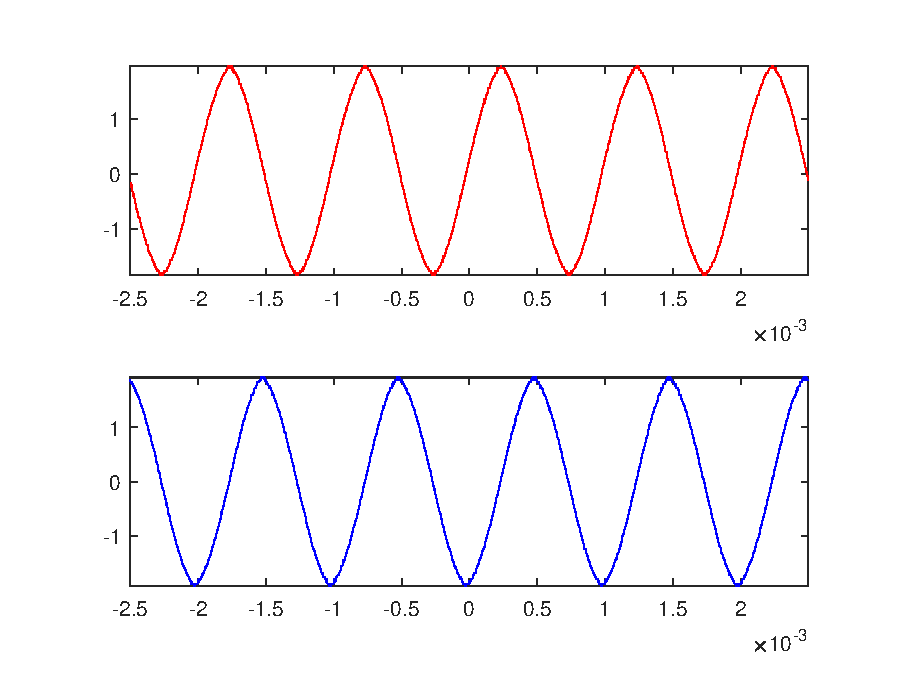
\includegraphics[width=.45\textwidth]{001}\\
(a)仿真软件中频信号&(b)示波器中频信号\\
\end{tabular}
\caption{中频信号}\label{zpxh}
\end{figure}
\subsubsection{基带信号}
基带信号的系统仿真图像与示波器波形见图\ref{jdxh}
。
\begin{figure}[htbp]
\centering
\begin{tabular}{cc}
\includegraphics[width=.55\textwidth]{TIM20190915233658}&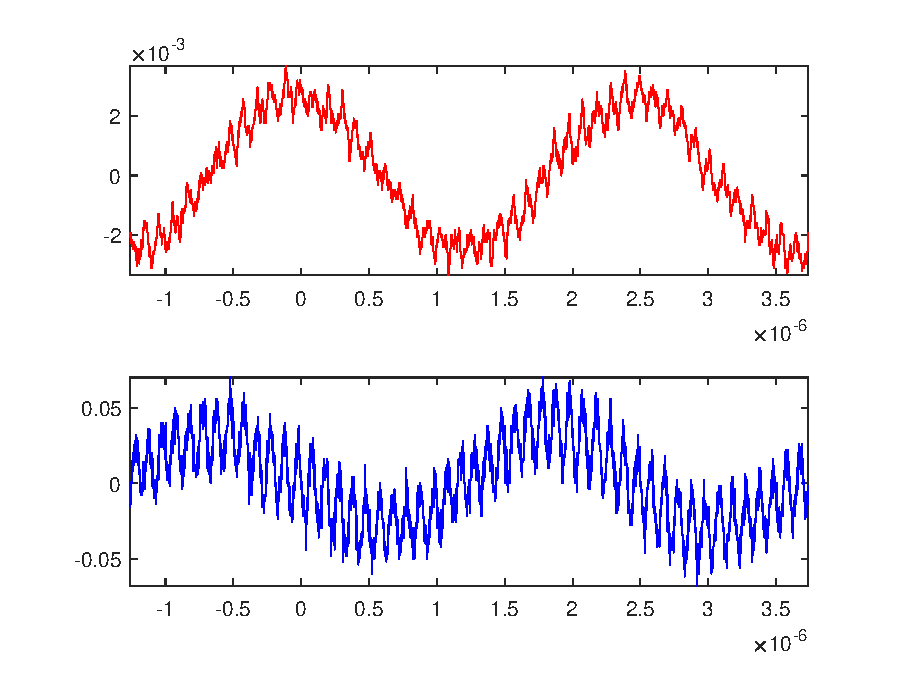
\includegraphics[width=.45\textwidth]{002}\\
(a)仿真软件基带信号&(b)示波器基带信号\\
\end{tabular}
\caption{基带信号}\label{jdxh}
\end{figure}
\subsubsection{脉压信号}
脉冲压缩信号的系统仿真图像与示波器波形见图\ref{myxh}
。
\begin{figure}[htbp]
\centering
\begin{tabular}{cc}
\includegraphics[width=.55\textwidth]{TIM20190915233929}&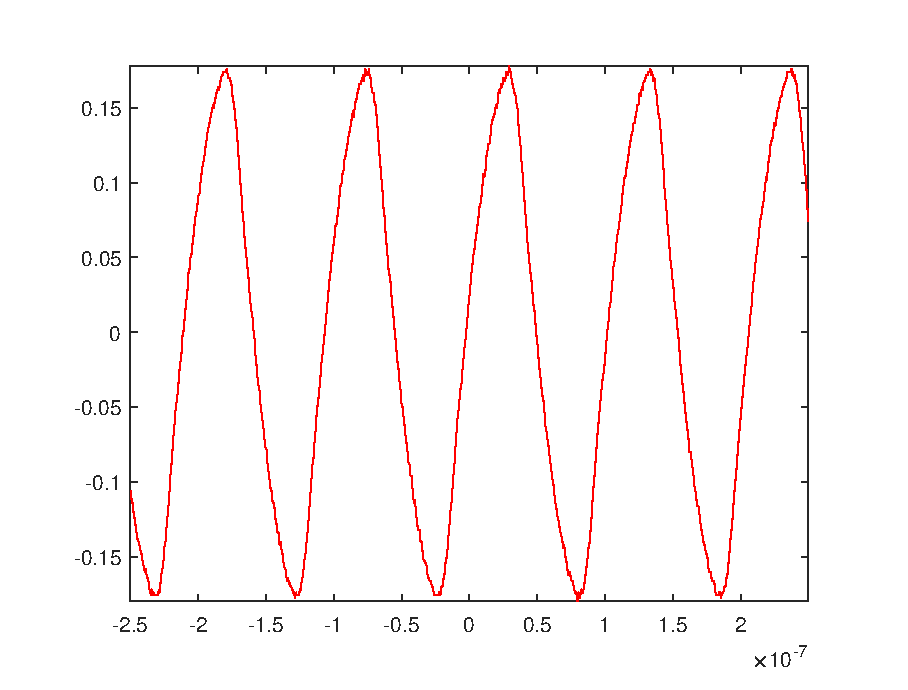
\includegraphics[width=.45\textwidth]{003}\\
(a)仿真软件脉压信号&(b)示波器脉压信号\\
\end{tabular}
\caption{脉压信号}\label{myxh}
\end{figure}
\subsection{双目标情况}
\subsubsection{距离分辨率}
由表\ref{tab:xtcsqk},系统理论的距离分辨率为15m。在仿真软件上进行仿真的情况如图\ref{jlfblxh}
所示。
\begin{figure}[htbp]
\centering
\begin{tabular}{cc}
\includegraphics[width=.5\textwidth]{TIM20190916000221}&\includegraphics[width=.5\textwidth]{TIM20190916000337}\\
(a)目标距离差为100m&(b)目标距离差为50m\\
\ &\ \\
\includegraphics[width=.5\textwidth]{TIM20190916002058}&\includegraphics[width=.5\textwidth]{TIM20190916002145}\\
(c)目标距离差为20m&(d)目标距离差为10m\\
\end{tabular}
\caption{距离分辨率仿真}\label{jlfblxh}
\end{figure}\par
由仿真图可知,当两者的目标大于距离分辨力时,系统可以区分两个目标,且距离差越大,越明显,当距离小于距离分辨力时,系统无法区分两个目标。
\subsubsection{速度分辨率}
由表\ref{tab:xtcsqk},系统理论的速度分辨率为2.93m/s。在仿真软件上实际进行仿真的情况如图\ref{sdfblxh}
所示。
\begin{figure}[htbp]
\centering
\begin{tabular}{cc}
\includegraphics[width=.5\textwidth]{TIM20190916004903}&\includegraphics[width=.5\textwidth]{TIM20190916004815}\\
(a)目标速度差为20m/s&(b)目标速度差为10m/s\\
\ &\ \\
\includegraphics[width=.5\textwidth]{TIM20190916003254}&\includegraphics[width=.5\textwidth]{TIM20190916004656}\\
(c)目标速度差为5m/s&(d)目标速度差为3m/s\\
\end{tabular}
\caption{速度分辨率仿真}\label{sdfblxh}
\end{figure}\par
由仿真图可知,当两者的目标大于速度分辨力时,系统可以区分两个目标,且速度差越大,越明显;实际仿真过程中,当速度小于4m/s时,系统已无法明确区分两个目标。
\section{MATLAB仿真}
\setcounter{table}{0}\setcounter{figure}{0}\setcounter{equation}{0}
针对实验所设计的LFM脉冲雷达系统,在MATLAB上进行了相应的仿真研究,加入噪声后,仿真所得到的各个波形如图\ref{jidaibox}$-$\ref{maiyabox}
所示。
\begin{figure}[htbp]
  \centering
  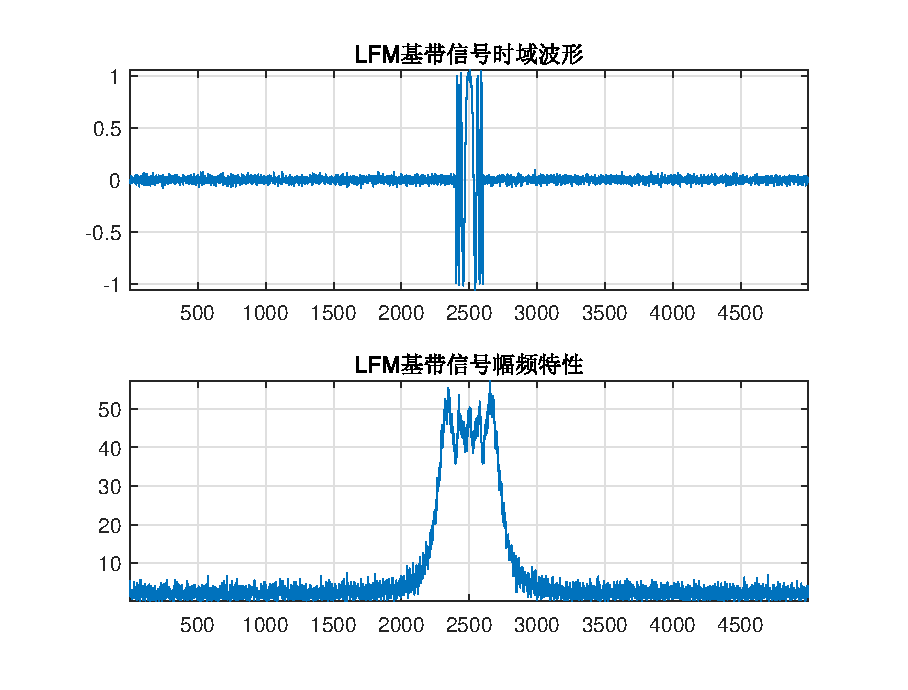
\includegraphics[width=.8\textwidth]{jidaibox}
  \caption{基带信号}\label{jidaibox}
\end{figure}
\begin{figure}[htbp]
  \centering
  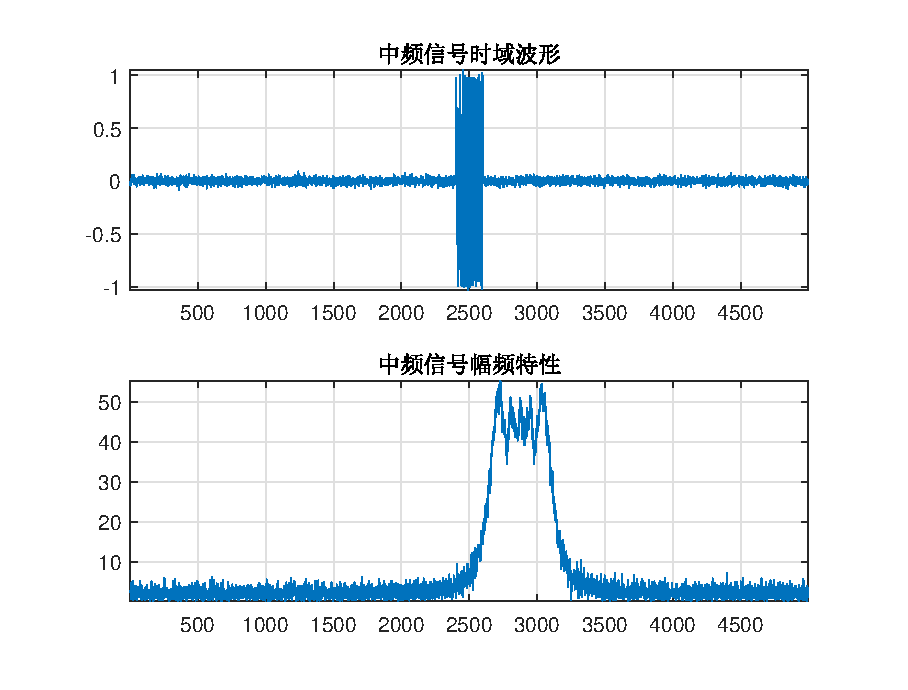
\includegraphics[width=.8\textwidth]{zhongpinbox}
  \caption{中频信号}\label{zhongpinbox}
\end{figure}
\begin{figure}[htbp]
  \centering
  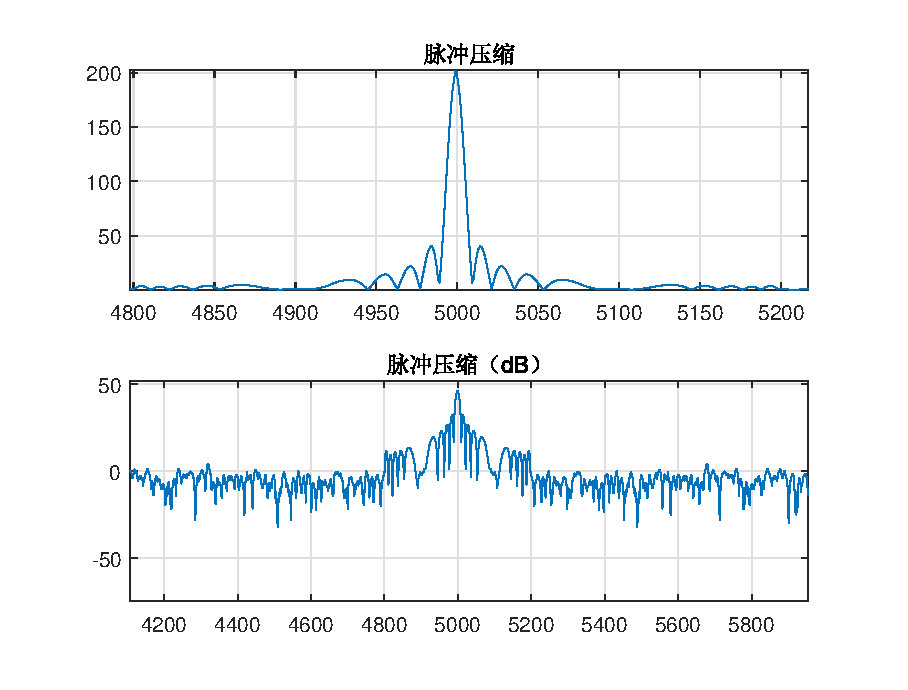
\includegraphics[width=.8\textwidth]{maiyabox}
  \caption{脉压信号}\label{maiyabox}
\end{figure}

\section{实验感想与体会}
\setcounter{table}{0}\setcounter{figure}{0}\setcounter{equation}{0}
在本次实验中,我充分体会到了理论与实际相结合的重要性。\par
实验过程中,同时也锻炼了我的实际动手能力,例如示波器的调试、硬件的连接等等。
\par
事实上,MATLAB仿真的内容在卓工的《信号检测与估计》中有做过类似的内容,但结合实物进行雷达系统设计实验还属首次,在实验过程中也遇到了一些问题,主要是与实验箱和示波器有关。设置目标RCS为0.01$m^2$时,虽然在仿真系统上可以观察到相应波形,但无法在示波器上观察到。即使调整信噪比和发射功率也仍然无效,推测是雷达目标截面积过小,噪声使得信号达不到示波器能检测的阈值。增加RCS至0.05$m^2$后,可以在示波器上观察到波形。
\par
本次仿真实验结合了雷达原理、数字信号处理等课程的内容,通过独立自主地完成本次仿真实验,我基本上了解、明白了雷达信号对于信号的识别过程。\par
当然,实验也存在令人遗憾的内容。由于对示波器不够熟悉,尤其是触发电平功能不够了解,在最后的考核中并没有取得十分理想的成绩。\par
最后,我要感谢在实验中给予我帮助的李洪涛老师,以及在实验过程中与我一同讨论的卢铭同学。
\section{附录:matlab代码}
\begin{lstlisting}[language=matlab]
clc;
clear;
B=10e6;             %带宽
T=5e-5;             %脉冲重复周期
Tau=2e-6;           %脉宽
Fc=16e9;            %载频
F0=7.5e6;
SNRi=30;            %输入信噪比
V=0;              %目标速度
A=0.01;           %目标幅度
R=0;            %目标距离
%******************常数或中间参数*******************
D=Tau/T;            %占空比
K=B/Tau;              %线性调频斜率
Fs=100e6;             %采样频率
Ts=1/Fs;            %采样周期
C=3e8;              %光速C
%******************线性调频信号***************
N=round(T/Ts);
t1=linspace(-Tau/2,Tau/2,N*D);
St_1=exp(2*j*pi*(F0*t1+0.5*K*t1.^2));
St_0=exp(2*j*pi*(+0.5*K*t1.^2));
N1=round(N*(1-D)/2);
zero=zeros(1,N1);%补零
St_0=[zero,St_0,zero];
St_1=[zero,St_1,zero];
St_0=awgn(St_0,SNRi);%加入噪声
St_1=awgn(St_1,SNRi);
%LFM时域波形
 figure(1);
 subplot(2,1,1)
 plot(real(St_0));
 title('LFM基带信号时域波形');
 grid on;axis tight;
%LFM频域波形
 figure(1);
 subplot(2,1,2)
 fftshift(abs(fft(St_0)));
 St_FFT_0=fftshift(abs(fft(St_0)));
 plot(St_FFT_0);
 title('LFM基带信号幅频特性');
 grid on;axis tight;
%中频信号时域
figure(2);
 subplot(2,1,1)
 plot(real(St_1));
 title('中频信号时域波形');
 grid on;axis tight;
%中频信号频域
 figure(2);
 subplot(2,1,2)
 fftshift(abs(fft(St_1)));
 St_FFT_1=fftshift(abs(fft(St_1)));
 plot(St_FFT_1);
 title('中频信号幅频特性');
 grid on;axis tight;
%***************匹配滤波*********************
Ht_0=fliplr(St_0);
Ht=conj(Ht_0);
Sot=conv(St_0,Ht);
Z0=abs(Sot);
%匹配滤波
 figure(3)
 subplot(2,1,1)
 plot(Z0);
 grid on;axis tight;
 title('脉冲压缩');
%匹配滤波dB
 figure(3)
 subplot(2,1,2)
Z1=20*log10(Z0);
 plot(Z1);
 grid on;axis tight;
 title('脉冲压缩(dB)');

\end{lstlisting}
\end{document}
